%%%%%%%%%%%%%%%%%%%%%%% file typeinst.tex %%%%%%%%%%%%%%%%%%%%%%%%%
% VINSTITUTO POLITÉCNICO NACIONAL
% CENTRO DE INVESTIGACIÓN EN COMPUTACIÓN
% PROTOCOLO PARA REGISTRO DE TEMA DE TESIS
% MAESTRÍA EN CIENCIAS DE LA COMPUTACIÓN
% MAESTRÍA EN CIENCIAS EN INGENIERÍA DE CÓMPUTO
% SEMESTRE B22
%%%%%%%%%%%%%%%%%%%%%%%%%%%%%%%%%%%%%%%%%%%%%%%%%%%%%%%%%%%%%%%%%%%
\documentclass[runningheads,a4paper]{llncs}

\usepackage[utf8]{inputenc}
\usepackage{amssymb}
\usepackage{pgfgantt}
\usepackage{graphicx}
\usepackage{url}
\usepackage{biblatex}
\usepackage{graphicx}
\graphicspath{ {./} }
\usepackage{geometry}
    \geometry{
    a4paper,
    total={170mm,257mm},
    left=20mm,
    top=20mm,
}

\newcommand{\keywords}[1]{\par\addvspace\baselineskip
\noindent\keywordname\enspace\ignorespaces#1}

\begin{document}

\title{
    Generadores de Señales de Reloj Para Procesadores SoC
}

\author{
    Luis Juventino Velasquez Hidalgo,\\
    M.Osvaldo Espinosa Sosa,\\
    Dr. Victor Hugo Ponce Ponce
}

\urldef{\mailsa}\path|lvelasquezh2024@cic.ipn.mx|
\urldef{\mailsb}\path|{vponce@cic.ipn.mx, espinosa@cic.ipn.mx}@cic.ipn.mx|    
\institute{
    Centro de Investigación en Computación\\
    Av. Juan de Dios Bátiz, esq. M
    guel Othón de Mendizábal\\
    Col. Nueva Industrial Vallejo, Alcaldía Gustavo A. Madero, C.P. 07738, CDMX\\
    Unidad Profesional Adolfo López Matéos (Zacaténco)\\
    \mailsa\\
    \mailsb\\
    \url{http://www.cic.ipn.mx}
}
\maketitle

\begin{abstract} 
    Las señales de reloj son fundamentales para el funcionamiento de todos los procesadores. Este trabajo explora la creacion de una señal de reloj digital utilizando un \textit{Phase-lock loop} \textbf{(PLL)}. 

    El area de \textit{System on Chip} \textbf{(SoC)} es un campo muy cerrado, pero es un campo muy amplio y requerido para distintas aplicaciones. Por lo que uno de los objetivos del presente trabajo es diseñar el PLL en un lenguaje de descripción de hardware para generar una referencia de dichas tecnologias.

    \keywords{FPGA, SoC, Sistemas Embebidos, Microprocesadores, PLL, Microtecnologias}
\end{abstract}

\section{Introducción}

Un procesador es un circuito integrado encargado de ejecutar instrucciones y procesar datos en un sistema informático. Se le llama SoC a un dispositivo que integra todos los componentes esenciales de un sistema, por ejemplo; memoria, controladores, procesador y otros bloques funcionales. El avance de las microtecnologías ha echo que para concretar el diseño de un SoC sea necesario usar un \textit{hardware description language} \textbf{(HDL)}${}^3$ para describir el comportamiento del sistema en lugar de describir la circuitería necesaria.

    El reloj es uno de los componente principales en le diseño de SoC's. El reloj se encarga de generar señales periódicas estables esenciales para coordinar todos los componentes del sistema. La linea de investigación de la propuesta de tesis está encaminada al desarrollo de un reloj integrable a un SoC.\\

    En los SoC los relojes usualmente se implementa usando sensores \textit{On-chip}, generadores de reloj \textit{On-chip}${}^1$ o haciendo uso de PLL's siendo estos últimos en los que se enfoca la propuesta de tesis. El principal problema es que el ecosistema de desarrollo en HDL es muy cerrado y es común que los componentes individuales no sean transparentes. La propuesta de está tesis es \textbf{crear un diseño de reloj en HDL} para uso general y de acceso libre.\\

   Un PLL se evalúa principalmente con dos metricas: \textit{jitter} y \textit{Phase noise} (Ruido de fase)${}^4$. Como la finalidad del PLL es fungir como reloj, a estas metricas se le añade la frecuencia maxima.
    El jitter; ocasionalmente referido como \textit{time interval error}, es una medida estadística de la desviación entre los flancos de la señal cuadrada ideal comparado con la señal real. Al ser una medida estadística se necesita de un muestreo a partir del cual se caracteriza al jitter y poder calcular, por ejemplo; la desviación máxima, el promedio aritmético de la desviación y la desviación del promedio. Por otro, el ruido de fase es una varianza en la magnitud horizontal de la onda. A diferencia del ruido aditivo el cual solo afecta a la amplitud de la onda, la varianza horizontal puede cambiar el periodo de la señal deseada.

    En un articulo publicado en el 2022${}^5$ se reseñaron en total 144 publicaciones de la \textit{ISSCC} y \textit{VLSI}, dando como resultado que 38\% de las publicaciones hablan de \textit{ADPLL}, 15\% sobre \textit{SSPLL},18\% de \textit{ILPLL} , 7\% de \textit{MDLL} y el 22\% restante de otros diseños.
    Uno de los resultados que se obtuvo en el articulo mencionado es que los avances en el diseño de PLL se pueden dividir en 3 categorías: aumentar la frecuencia conservando el consumo de energía, aumentar la frecuencia manteniendo la relación de frecuencia-consumo de energía, aumentar la frecuencia manteniendo el jitter normalizado\\

    Existen muchas implementaciones de PLL, pero los componentes fundamentales son; el \textit{Error detector} compuesto por un detector de frecuencia de fase y un regulador de voltaje, un \textit{Loop Filter} para suavizar la señal de error generado por el \textit{Error detector}, un \textit{Voltage-controlled oscillator} (\textbf{VCO}) encargado de ajustar la frecuencia en función de la señal de error del \textit{Error detector} para compararla con la señal deseada y un \textit{feedback divider} encargado de regular la señal del \textit{VCO} para que este en la misma fase y frecuencia que la señal de referencia.\\ 


\begin{figure}[t]
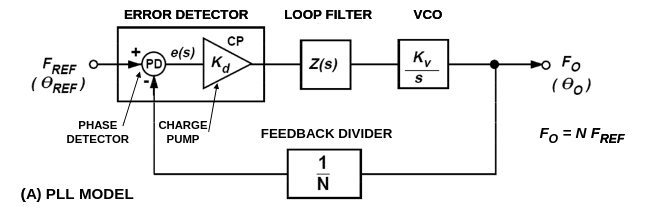
\includegraphics[width=8cm]{PLL.png}
\centering
\caption{Arquitectura base de un PLL. Rescatado de${}^6$}
\end{figure}

    De la arquitectura base se desprenden implementaciones como en ${}^7$ la cual añade; para la implementación de un SoC, un control de voltaje antes del \textit{VCO} para disminuir el efecto del ruido generado por todos los componentes digitales existentes en el chip. Aumentando el consumo de energía pero reduciendo el jitter.

    Cada problema que necesite una implementación requiere especificaciones diferentes. Sera trabajo de la tesis definir si el reloj estará enfocado a un uso especifico o a uno más general y bajo que condiciones otra tecnología se adaptaría mejor al problema. Una de los factores que afectan el rendimiento del reloj en un SoC es la distribución del mismo, al trabajar con frecuencias muy altas la frecuencia llega con un desface diferente en cada dispositivo, es por eso que hay distintas arquitecturas para la correcta distribuccion de la señal de reloj, por ejemplo: \textit{ring clock},\textit{tree-clock} y \textit{mesh clock}. Es trabajo de la tesis saber con que arquitectura se acomoda mejor el reloj diseñado\\


\section{Características y generalidades}

Cada implementación de un SoC está caracterizado por un conjunto de restricciones, como lo es el tamaño del chip, el consumo energético y la frecuencia a la que debe trabajar el sistema. Dichas restricciones pueden ser parte del problema o consecuencia de los componentes individuales a usar. En lo que concierne al reloj; ademas de las métricas ya mencionadas, es necesario pensar en la distribución de todos los componentes que del SoC para asegurar que la señal llegue en sincronía a cada elemento que lo conforma.\\

Para poder cumplir con las métricas necesarias del reloj se han desarollado las tecnicas ya mencionadas, las cuales son: \textit{ADPLL}, \textit{SSPLL}, \textit{ILPLL} y \textit{MDLL}. También ha sido necesario desarrollar en la arquitectura necesaria para llevar la señal de reloj a cada componente del SoC, como las ya mencionadas: \textit{ring clock}, \textit{tree clock} y {mesh clock}. Es prudente mencionar que algunas técnicas de PLL se integran mejor a arquitecturas especificas, como lo es el SSPLL con el \textit{ring clock} . El entregable propuesto es el diseño de un PLL y su implementación en una arquitectura SoC pensando en las necesidades más generales de un sistema: integración de cpu , memoria y puertos perifericos, bajo consumo de energía, bajo costo de producción, tamaño reducido y respuesta en tiempo real. 

La relevancia de dicho trabajo radica en la necesidad de generar el conocimiento de cómo diseñar SoC's, siendo la integración del reloj el primer paso del proceso. Dicha integración implica un estudio para relacionar las necesidades del SoC con el diseño del PLL. 

%Describir como se resuelve el problema a priori.
%Esquema de trabajo
% 'se tiene que ver claramente qué de nuevo se va a realizar con respecto a lo que ya se ha hecho Definir productos y entregables, asi como derivados'

\subsection{Objetivo General:}
\paragraph{Diseñar un reloj en lenguaje DHL}
\paragraph{Investigar las diferentes tecnologías en el diseño de PLL e identificar sus ventajas y casos de uso}
\paragraph{Investigar arquitecturas para integrar un reloj en circuitos SoC e identificar sus casos de uso}
\paragraph{Identificar posibles implementaciones de un SoC en problemas actuales}

\subsection{Objetivos específicos:}
\paragraph{Integrar la señal del reloj con otros periféricos o circuitos. Por ejemplo, el procesador lagarto}
\paragraph{Caracterizar el reloj echo midiendo su frecuencia máxima, jitter y ruido de fase}


\subsection{Índice tentativo de la tesis:}
\begin{itemize}
\item Introduccion
\item Necesidades de un SoC
\item Fundamentos de un PLL
\item Diseño tradicional de PLL's
\item Arquitecturas reloj en SoC 
\item Nuevas tecnologias en el diseño de PLL's
\begin{itemize}
    \item ADPLL
    \item SSPLL
    \item ILPLL
    \item MDLL
\end{itemize}
\item Implementación y rendimiento de un SoC
\item Conclusiones
\end{itemize}


\section{Aspectos importantes a destacar del trabajo de tesis}
% XXX(Atencion) No pedí apoyo al director de tesis
\begin{itemize}
\settowidth{\leftmargin}{{\Large$\circ$}}\advance\leftmargin\labelsep
\itemsep8pt\relax
\renewcommand\labelitemi{{\lower1.5pt\hbox{\Large$\circ$}}}

     \item Un reloj es necesario para implementar un sistema embebido y actualmente el laboratorio de Microse no cuenta con el diseño de uno

     \item Una de las tendencias es el diseño de relojes totalmente digitales(\textit{ADPLL}), dedicarle tiempo a investigar esta tecnología ayuda al laboratorio a estar actualizado con los avances en el campo.

     \item La arquitectura del reloj de un SoC es un subconjunto del diseño de un SoC: a su vez, El diseño de un SoC es un campo de estudio importante en el campo de sistemas embebidos.

 \end{itemize}
Al finalizar la tesis, el alumno deberá ser capas de; dado un problema, identificar las necesidades de un SoC. Además de obtener habilidades técnicas para aumentar la frecuencia de un reloj, reducir la necesidades energéticas del mismo y poder asegurar que la señal del reloj llegue sincronizada a todos los componentes. 

\section{Plan de trabajo y cronograma}

Enumere y describa sucintamente las acciones y actividades que desarrollará para lograr los objetivos propuestos, así como los productos que se generarán como fruto del desarrollo de las actividades. 
\begin{table}
\begin{center}
\begin{tabular}{|p{2cm}|p{5cm}|p{5cm}|} 
\hline\noalign{\smallskip}
Consecutivo & Actividades o acciones a desarrollar & Productos Esperados\\

\noalign{\smallskip}
\hline
\noalign{\smallskip}
1& Hacer un estudio de las técnicas existentes para implementar circuitos PLL & Una tabla comparativa con las ventajas, desventajas y especificaciones de cada circuito \\\hline
2&Diseñar las versiones digital y analógica del circuito PLL & Diseño conceptual de cada reloj \\\hline
3&Utilizar software de diseño y simulación para obtener las versiones de los circuitos PLL & Diseños en HDL de los circuitos\\\hline
4&Implementar el PLL en una placa de desarrollo & Un PLL funcional integrado a una placa de desarollo \\\hline
5&Obtener el lay-out de los circuitos propuestos & Diseño del PLL en una placa fisica \\\hline
6&Hacer análisis de los circuitos obtenidos & Conclusiones preliminares de la tesis\\\hline
7&Escritura de la tesis & La tesis \\\hline
8&Presentación del examen de puerta cerrada. & Evaluación de las conclusiones mostradas en la tesis \\\hline
\end{tabular}
\end{center}
\end{table}

\subsection{Plan de estudios }
Debe señalar los meses estimados de inicio y término de cada una de las actividades descritas en el plan de trabajo, a partir de la fecha de presentación de esta solicitud.

\begin{ganttchart}[
canvas/.append style={fill=none, draw=black!5, line width=.75pt},
hgrid style/.style={draw=black!5, line width=.75pt},
vgrid={*1{draw=black!5, line width=.75pt}},
today=1,
today rule/.style={
draw=black!64,
dash pattern=on 3.5pt off 4.5pt,
line width=1.5pt
},
today label font=\small\bfseries,
title/.style={draw=none, fill=none},
title label font=\bfseries\footnotesize,
title label node/.append style={below=7pt},
include title in canvas=false,
bar label font=\mdseries\small\color{black!70},
bar label node/.append style={left=2cm},
bar/.append style={draw=none, fill=black!63},
bar incomplete/.append style={fill=barblue},
group incomplete/.append style={fill=groupblue},
group left shift=0,
group right shift=0,
group height=.5,
group peaks tip position=0,
group label node/.append style={left=.6cm},
group progress label font=\bfseries\small,
link/.style={-latex, line width=1.5pt, linkred},
link label font=\scriptsize\bfseries,
link label node/.append style={below left=-2pt and 0pt},
]{1}{19}
\gantttitle{2do Semestre}{7}
\gantttitle{3er Semestre}{6}
\gantttitle{4to Semestre}{6} \\
\ganttbar[
]{\textbf{Actividad 1}}{1}{3} \\
\ganttbar[
]{\textbf{Actividad 2}}{3}{7} \\
\ganttbar[
]{\textbf{Actividad 3}}{6}{12} \\
\ganttbar[
]{\textbf{Actividad 4}}{9}{14} \\
\ganttbar[
]{\textbf{Actividad 5}}{11}{15} \\
\ganttbar[
]{\textbf{Actividad 6}}{14}{17} \\
\ganttbar[
]{\textbf{Actividad 7}}{3}{19} \\
\ganttmilestone{\textbf{Actividad 8}}{19}{19}  \\

\ganttlink[link type=f-s]{bar1}{bar2}
\ganttlink[link type=f-s]{bar4}{bar5}
\end{ganttchart}


\section{Recursos requeridos de hardware y software}
\begin{itemize}
\item Computadora de desarrollo
\item Software de desarrollo de HDL
\item Placa de desarrollo
 \end{itemize}



\section{Estancia de investigación}
Me gustaría hacer una estancia de investigación en el ultimo semestre. Aun no hay un grupo de trabajo identificado en el que pueda desarrollarme. \\ 


\break
\section{Plan de UA que cursará}
\begin{table}
\begin{center}
 \begin{tabular}{|l|l|}
Primer Semestre & Segundo Semestre\\
1. 15A7160 Matemáticas para las ciencias de la computación & 1. 15A7159 Diseño y Análisis de Algoritmos \\
2. 15A71761 Probabilidad, procesos aleatorios e inferencia & 2. 15A7162 Teoría de la Computación \\
3. 15A7203 Internet de las Cosas & 3. 15A7211 Lenguajes de Descripción de Hardware \\ 
4. 15A7228 Procesamiento digital de señales & 4. 15A7200 Identificación de Sistemas \\ 
5. 15A7215 Microtecnología y Arquitectura de Procesadores & 5. Tema de tesis\\ 
6. Seminario  \\
\hline\noalign{\smallskip}
Tercer Semestre & Cuarto Semestre\\

1. 15B7298 Diseño de Circuitos VLSI Avanzados & 1. Tema de tesis\\
2. 15A7194 Diseño de Sistemas VLSI & \\
3. 15A7240 Redes sociales y complejidad / Complex Social Networks & \\
4. Seminario III& \\
5. Tema de tesis & \\
\hline
\end{tabular}
\end{center}
\end{table}

\section{Comité tutorial propuesto}
\begin{itemize}
\item M. Osvaldo Espinosa Sosa
\item Dr. Victor Hugo Ponce Ponce
\item Dr. Hector Báez Medina
\item Dr. Herón Molina Lozano
 \end{itemize}


\section{Retribución social}
\begin{itemize}
    \item Presentar resultados de su investigación ante grupos sociales, productivos e instituciones 
    \item Colaborar en procesos de innovación social y tecnológica.
    \item Impartir cursos o talleres de formación e innovación social.
    \item Participar en foros de intercambio de experiencias sociales/institucionales
    \item Apoyar a los programas de posgrado registrados en el SNP para dar cursos, talleres, conferencias, etc., sobre los temas en los que se es experto
    \item Divulgar la ciencia y tecnología a niños y jóvenes, mediante cursos y pláticas.

 \end{itemize}



\section{NOTA ACLARATORIA}
El presente documento es representativo de que tanto el alumno, así como el(los) director(es) de tesis están de acuerdo en trabajar conjuntamente para cumplir los objetivos planteados en el mismo, quedando claro que el contenido de éste es pieza sustentante de las labores a desarrollar por ambas partes y que al momento de ser entregado a la coordinación del programa, queda de conformidad su desarrollo por los involucrados. Considerando además que la planeación presentada emana de una propuesta por parte del o los director(es) de tesis y es un trabajo a desarrollar por el asesorado cuya labor se considera como un recurso humano de apoyo a un investigador.

%\section*{References}

\break
\begin{thebibliography}{4}
    \bibitem{jour} Brackenbury, L. E. M., Plana, L. A., & Pepper, J. (2010). System-on-Chip Design and Implementation. IEEE Transactions on Education, 53(2), 272–281. doi:10.1109/te.2009.2014858 en \url{https://ieeexplore.ieee.org/abstract/document/5196691?casa_token=TpI81j-CHq4AAAAA:ILb9l6GoYXNWQbEPythUCDtK5P1gD1r4HOItcKHaa1guUkdviQkCzPEXMteGrnGGqSA2KhfANXdP}

    \bibitem{jour} Lech Jóźwiak(2001), Quality-driven design in the system-on-a-chip era: Why and how?, Journal of Systems Architecture en \url{https://www.sciencedirect.com/science/article/pii/S1383762100000461?casa_token=A_tME0kkXqAAAAAA:kexFmDn0pCK5R-u1-8HtNg5OipAboKdQQhrSq3JXLFyNBPwSGPyhPnqJm5v44uHy2IDGlExRLkVd}

    \bibitem{jour} Chakravarthi, V. S. (2022). A practical approach to VLSI system on chip (SoC) design A practical approach to VLSI system on chip (SoC) design (2nd ed.). doi:10.1007/978-3-031-18363-8 en \url{https://link.springer.com/book/10.1007/978-3-031-18363-8}

    \bibitem{jour} Fahim, A. (2004). Clock generators for SOC processors [PDF]. doi:10.1007/b117041 en \url{https://link.springer.com/book/10.1007/b117041}

    \bibitem{jour} Bae, W. (2022). Benchmark figure of merit extensions for low jitter phase locked loops inspired by new PLL architectures. IEEE Access: Practical Innovations, Open Solutions, 10, 80680–80694. doi:10.1109/access.2022.3195687 en \url{https://ieeexplore.ieee.org/abstract/document/9847207}

    \bibitem{jour} Analog Devices. (2010). Fundamentals of Phase Locked Loops (PLLs) en \url{https://www.analog.com/media/en/training-seminars/tutorials/MT-086.pdf}

    \bibitem{jour} Young, I. A., Greason, J. K., & Wong, K. L. (1992). A PLL clock generator with 5 to 110 MHz of lock range for microprocessors. IEEE Journal of Solid-State Circuits, 27(11), 1599–1607. doi:10.1109/4.165341 en \url{https://ieeexplore.ieee.org/document/165341}

\end{thebibliography}
\printbibliography

\end{document}
